\documentclass[DIV14]{scrartcl}
%\usepackage[margin = 2.5cm, a4paper]{geometry}
\usepackage{tikz}
\usetikzlibrary{calendar,positioning}
\newcommand{\calyear}{2016}
\newcommand{\mon}[1]{\calendar[dates = \calyear-#1-01
  to \calyear-#1-last] if (Sunday) [red];}
\pagestyle{empty}
\begin{document}
  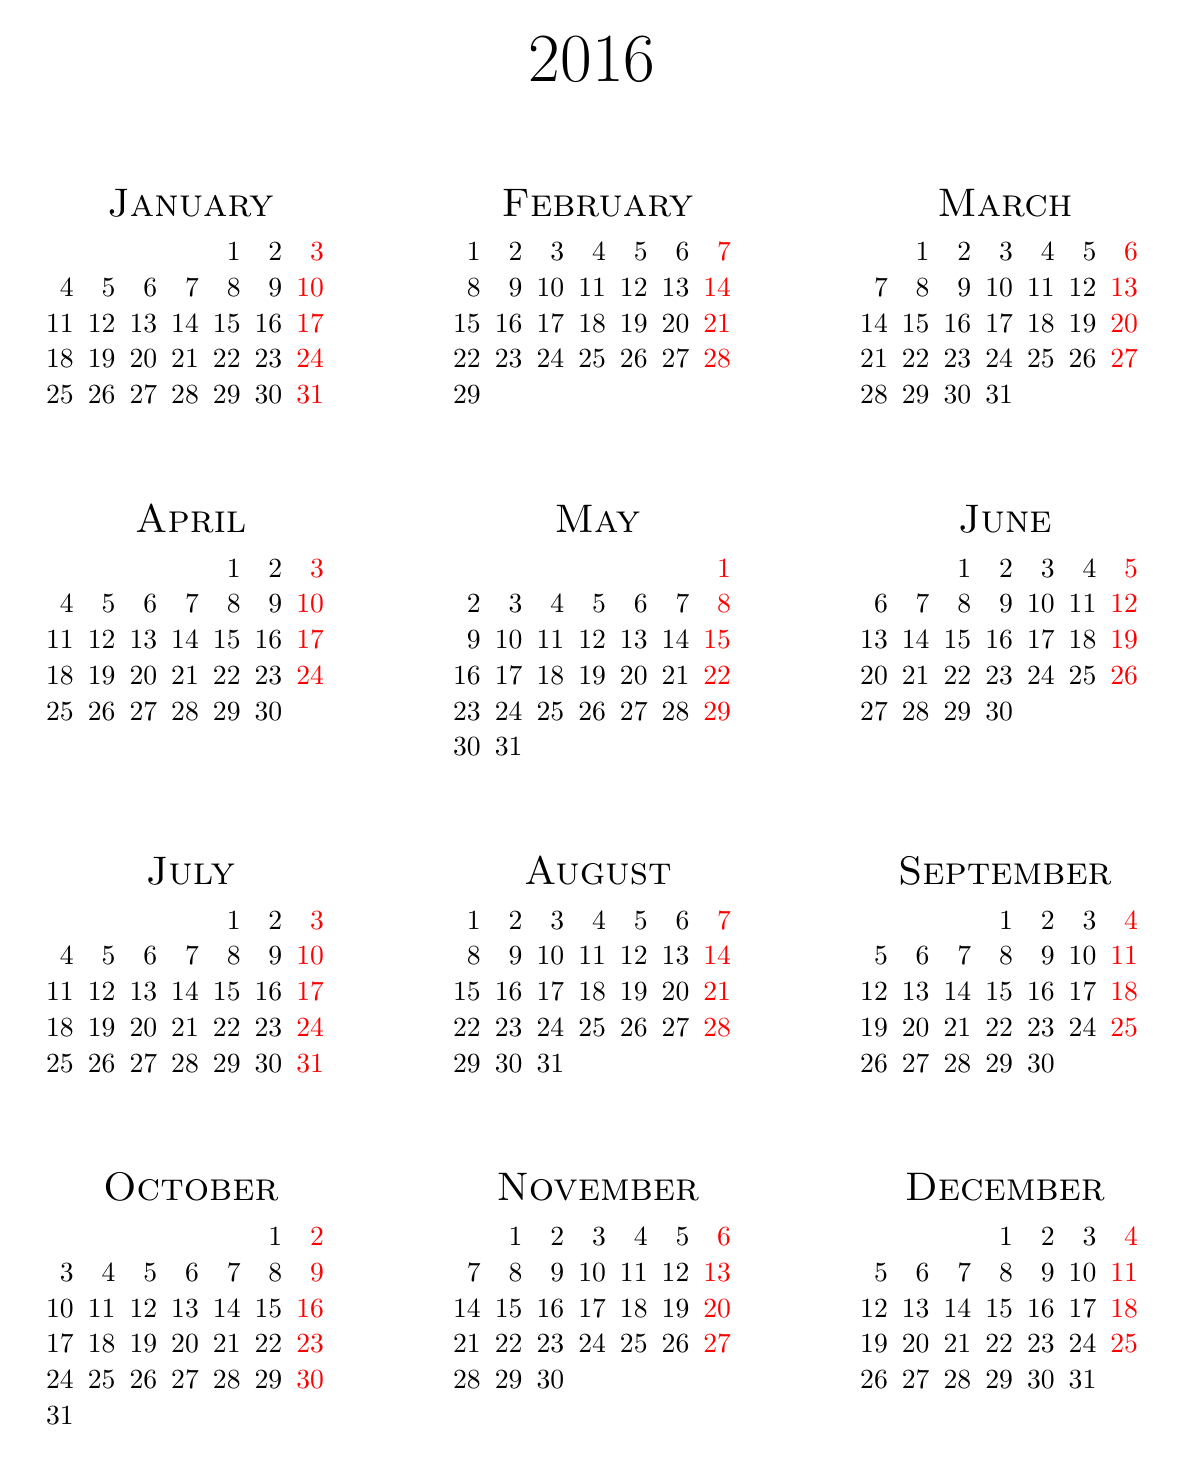
\begin{tikzpicture}[every calendar/.style = {
      month label above centered,
      month text = {\Large\textsc{\%mt}},
      week list,
    }]
    \matrix (Calendar) [column sep = 4em, row sep = 3em] {
      \mon{01} & \mon{02} & \mon{03} \\
      \mon{04} & \mon{05} & \mon{06} \\
      \mon{07} & \mon{08} & \mon{09} \\
      \mon{10} & \mon{11} & \mon{12} \\ };
    \node [above = 1cm of Calendar, font = \Huge] {\calyear};
  \end{tikzpicture}
\end{document}